\chapter{아날로그에서 디지털로}
디지털 데이터 스트림은 각각의 개별 구성 요소들로 쉽게 분해될 수 있는데, 이들은 보통 아날로그에서 대응되는 것들과 같은 역할을 한다.
아날로그와 디지털 비디오 영역을 설명하고 비교하는 동안 계속 이 관계를 사용할 것이다.
한번 아날로그와 디지털 비디오의 유사성을 이해하고 나면 HDTV를 다룰 수 있는데, 보통 이는 이에 대응되는 HD 아날로그 포맷의 디지털적 표현이다.
\\
NTSC와 PAL 비디오 신호들은 색의 삼원색인 빨강, 초록, 파랑 세 개의 카메라 채널의 합성인데, 행렬을 이용하여 합쳐져서 휘도를 만들고 이는 두 개의 색상 정보를 담고 있는 반송파 억압 변조의 결과물과 합쳐진다.
세 번쨰 단일 채널 컴포지트 전송 시스템은 SECAM 시스템인데, 이는 색상 정보를 전달하기 위해 한 쌍의 주파수 변조된 부반송파들을 이용한다.
스튜디오에서는 카메라의 RGB 감지 장치와 종단 디스플레이의 RGB 채널 사이의 어느 단에서도 신호가 NTSC, PAL 혹은 SECAM이 되어야 할 특별한 요구 조건은 없다.
NTSC, PAL 또는 SECAM에 대한 이해가 충분히 유용한 이상, 컴포지트 비디오에 대해서 더 많은 이해를 위해 투자하진 않을 것이다.

\section{RGB 컴포넌트 신호}
비디오 카메라는 이미지를 빛의 삼원색인 빨강, 초록, 파랑으로 분할한다. 카메라의 센서들은 이 각각의 단색 이미지들을 분리된 전기 신호로 변환한다.
그림의 왼쪽 끝과 최상단을 알려주는 동기 정보가 이 신호들에 추가된다. 디스플레이를 카메라와 동기화시키는 정보가 초록 채널에, 때로는 모든 채널에 더해지거나 아니면 별도로 전달된다.
\\
\begin{figure*}
    \centering
    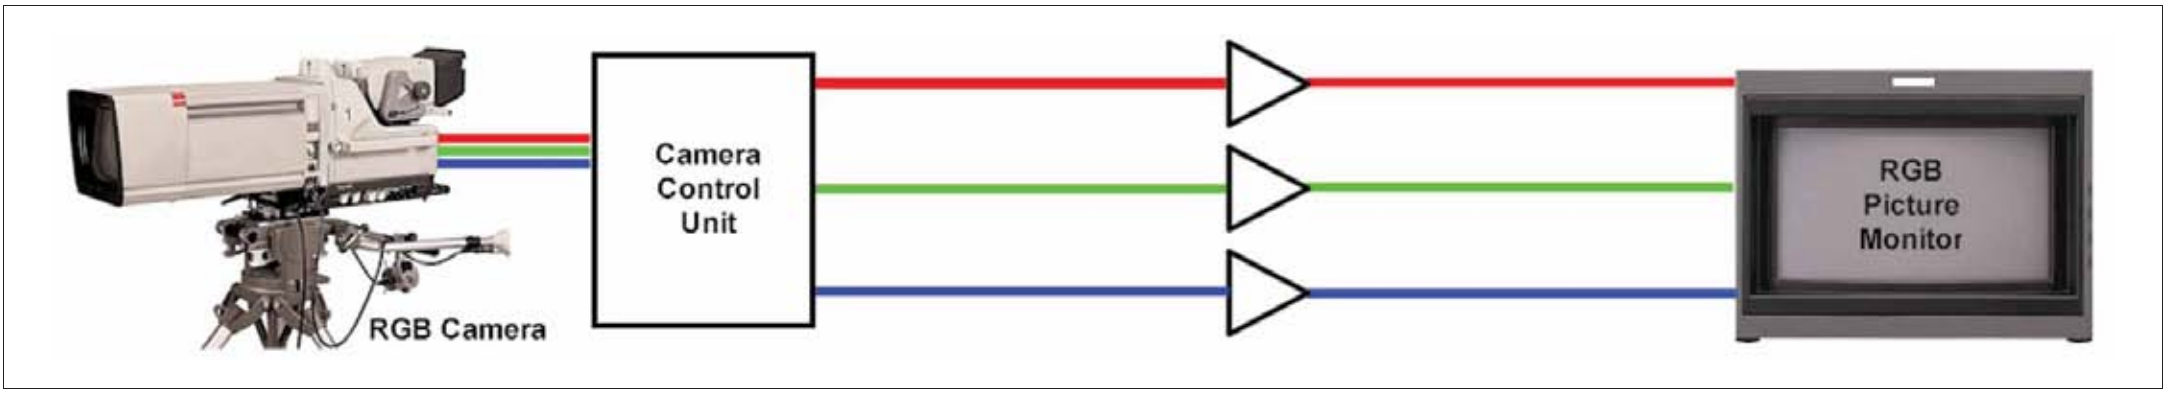
\includegraphics[width=\textwidth]{rgb camera to monitor direct.PNG}
    \caption{카메라에서 모니터까지 RGB 직접 연결}\label{fig:rgb camera to monitor direct}
\end{figure*}
가장 간단한 배선은 \figurename~\ref{fig:rgb camera to monitor direct}에 나와 있듯이 R, G, B를 카메라에서 그대로 뽑아서 모니터에 연결하는 것이다. 여러 선을 이용한 전송 시스템은 아날로그 SD에서나 HD 비디오에서나 같다.
여러 선을 이용한 연결은 작고, 영구적으로 구성된 부분 시스템에서 사용될 수 있을 것이다.
\\
이 방법은 카메라에서 디스플레이까지 고품질의 이미지를 만들어내지만, 신호를 세 분리된 채널로 전송하기 위해선 엔지니어가 각 채널이 신호를 처리할 때 같은 이득, 직류 오프셋, 시간 딜레이와 주파수 응답을 갖게 해야 한다.
각 채널의 이득이 다르거나 직류 오프셋에 오차가 생기면 최종 디스플레이 출력에서 미묘한 색상 변화가 일어날 것이다.
시스템에 타이밍 오차가 있을 수도 있는데, 이는 케이블 길이가 다르거나 각 신호를 카메라에서 디스플레이까지 라우팅하는 경로가 달라서 생길 수 있다.
이는 채널간 타이밍 오프셋을 만들 것이고 영상이 뭉개지게 만들 것이고, 심한 경우 이미지가 분리되어 여러 개가 나타날 것이다.
주파수 응답의 차이는 채널이 합쳐질 때 일시적인 악영향을 만들 것이다.
분명히 세 채널을 하나로 다룰 방법이 필요하다.
\\
\begin{figure*}[!h]
    \centering
    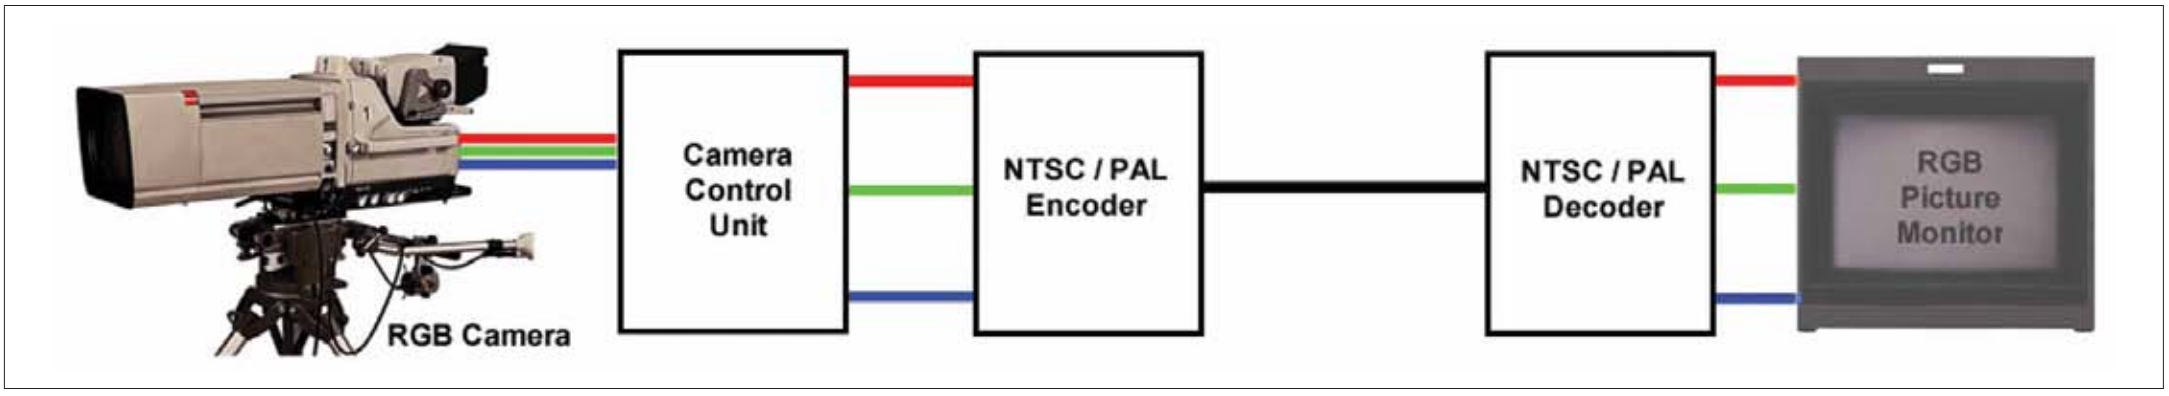
\includegraphics[width=\textwidth]{video encodeded into ntsc pal.PNG}
    \caption{단일 동축 케이블 전송을 위해 NTSC 또는 PAL로 인코딩된 비디오}\label{fig:video encodeded into ntsc pal}
\end{figure*}
NTSC나 PAL 인코더와 디코더를 \figurename~\ref{fig:video encodeded into ntsc pal}\와 같이 추가하는 것은 방송국 내에서 신호가 하나의 선으로 다뤄지는 것 외에는 단순화에 도움을 주지 못한다.
시스템 대역폭은 세 비디오 신호의 에너지를 4.2 MHz(NTSC)나 5.0에서 5.5 MHz(PAL) 내에서 다루기 적절하게 정해진다.
단일 선 구성은 비디오 라우팅을 쉽게 해 주지만, 더 먼 경로에 대해서 주파수 응답과 타이밍 문제를 고려해야 한다.
NTSC와 PAL 신호 모두에서 색상차와 휘도는 4.2 MHz(NTSC) 또는 5.0이나 5.5 MHz(PAL)의 대역폭을 공유하므로, 여러 번의 인코딩과 디코딩은 피해야 한다.
(역주: 좁은 대역폭 안에 신호가 들어가므로 열화를 피해야 함)
\\
\begin{figure*}[!t]
    \centering
    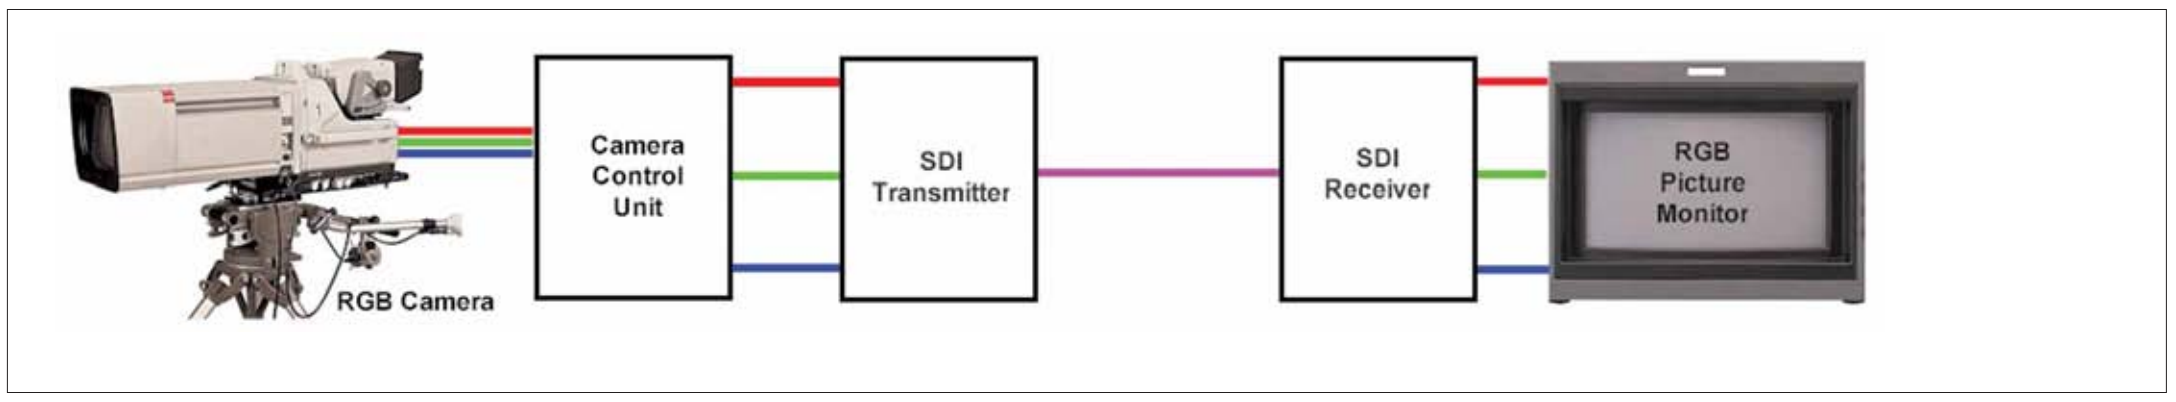
\includegraphics[width=\textwidth]{digital no degradation.PNG}
    \caption{디지털 전송에서는 아날로그적 신호 열화가 발생하지 않는다}\label{fig:digital no degradation}
\end{figure*}
위의 시스템에서 NTSC/PAL 인코더와 디코더를 컴포넌트 디지털 인코더와 디코더로 대체함으로써 \figurename~\ref{fig:digital no degradation}의 구성은 더 복잡하지도 않으면서 더 좋은 성능을 보인다.
하나의 동축 케이블에 들어있는 에너지는 SD 신호일 경우 270 Mb/s, HD 신호일 경우 1.485 Gb/s 이상의 속도이다.
SD 신호는 전통적인 방송 텔레비전 채널을 통한 전송을 하기 위해 아날로그 NTSC나 PAL로 변환될 수 있다.
HD 신호는 기존의 NTSC나 PAL 채널의 대역폭에 맞춰져서 공중파로 전송되기 위해서 압축되어야 한다.

\section{감마 보정}
비디오 신호를 다룰 때 고려해야 할 아날로그 요소는 비디오 디스플레이는 장면의 각 요소들의 밝기를 정확하게 표현한다는 생각이다.
음극선관(CRT) 디스플레이는 근본적으로 비선형 장치로서, 디스플레이에 가해지는 전압은 비선형적인 함수에 따라 정해지는 빛의 양으로 출력된다.
이 함수가 장치의 감마이다. 선형적인 응답을 얻기 위해서, TV 시스템 내에서 보정 요소가 가해져야 한다.
따라서, 카메라의 RGB 신호는 CRT의 역함수에 의해서 감마 보정이 이루어진다. 감마 보정된 신호는 R', G', B'와 같이 프라임(')마크가 붙어서 감지 장치에서 디스플레이로의 전달 함수에 대한 보정이 들어갔음을 나타낸다.
프라임 마크가 귀찮고, 때로 부적절하게 생략되긴 하지만, 표준 문서를 따르기 위해서 이 글에서 계속 사용될 것이다.
\\
LCD와 PDP가 보편적인 오늘날에는(역주: 이 글이 처음 쓰인 지 꽤 시간이 지났다) 감마 보정이 더이상 필요 없을 것이라고 생각될 수도 있다.
하지만, 인간의 밝기에 대한 시각 반응도 지수함수적인데, 약 1/3승을 따른다. 가장 좋은 명암 표현과 신호대잡음비(S/N, SNR)을 위해서 비디오 인코딩은 같은 지수함수를 이용한다. 이를 인지적 코딩이라고 한다.

\section{감마 보정은 CRT 반응에 대한 보정 이상을 의미한다}
CRT를 위한 감마 보정은 거의 최적의 인지적 보정이다. 이러한 이유로, 감마 보정 장치에 의해 보정 요소가 있는 시스템을 평가할 때는 유의해야 한다.
\\
\begin{figure*}
    \centering
    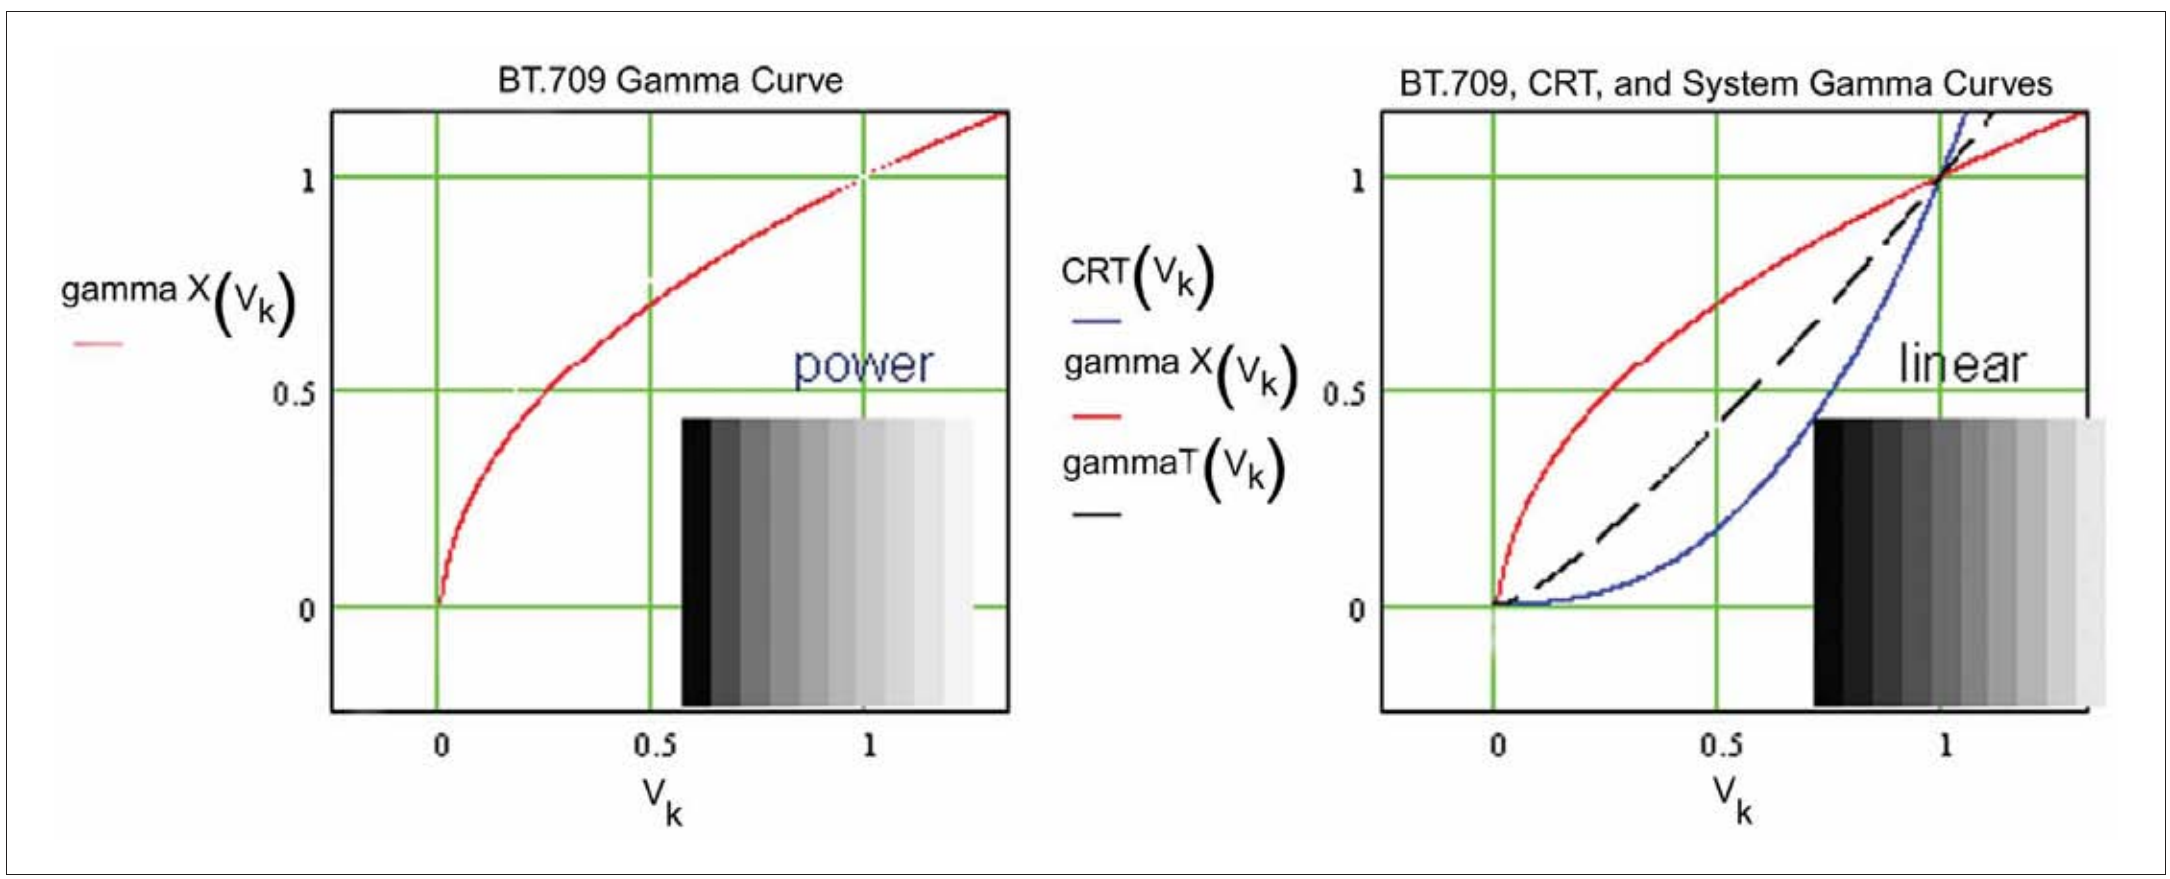
\includegraphics[width=\textwidth]{bt 709 gamma.PNG}
    \caption{BT.709 감마 보정은 CRT 디스플레이의 응답을 보정한다}\label{fig:bt 709 gamma}
\end{figure*}
\figurename~\ref{fig:bt 709 gamma}\는 ITU-R BT.709 표준에 따른 0.45승을 이용한 감마 보정을 보여주는데, 이 표준은 디지털 HD 비디오에 대한 보편적인 표준이다.
이 감마 보정은 CRT의 비선형성 교정과 인지적 코딩을 위해서 카메라에 적용된다. CRT의 비선형성은 2.2에서 2.6의 지수승을 갖는 지수함수이고, 대부분의 CRT는 2.5의 지수승을 갖는다.
최종적인 전체 시스템의 감마는 약 1.2로 일반적인 시청 환경에서 거의 이상적인 값이다. 이 응답은 대략적으로 인간의 밝기 인지 특성에 적합하고, 결과적으로 비디오가 전송을 위해 디지털화될 때에 필요한 비트 수를 줄여준다.

\section{R'G'B'신호의 휘도와 색상차 신호로의 변환}
빨강, 초록, 파랑의 비디오 요소들은 카메라의 감지 장치의 근본적인 것들이고 비디오 색상을 다룰 때 거의 항상 이용된다.
하지만 RGb는 비디오 처리를 할 때 이미지를 전달하는 가장 대역폭 효율적인 방법은 아닌데 이는 세 신호가 모두 같은 대역폭을 가져야 하기 때문이다.
인간의 시각은 색의 변화보다 밝기의 변화에 더 민감하고, 이를 이용해서 휘도 정보에 전체 대역폭을 할당하고 색차 신호들에는 남는 공간을 할당하는 방법을 통해서 대역폭 효율을 올릴 수 있다.
\\
비디오 신호 요소들을 휘도와 색차 값으로 처리하는 것은 전달되어야 하는 정보량을 줄여준다. 밝기와 신호의 세부 표현을 담당하는 휘도 채널(Y')에 전체 대역폭을 할당함으로써, 두 개의 색차 채널(R'-Y'와 B'-Y')은 휘도 채널 대역폭의 절반 정도만 사용해도 충분한 색 정보를 제공할 수 있다.
이를 이용해서 간단한 선형 행렬로 R'G'B'와 Y',R'-Y',B'-Y'를 상호 변환할 수 있다. 색차 신호 채널의 대역폭 제한은 행렬을 이용해서 할 수 있다.
채널이 디스플레이에서 R'G'B'로 복원될 때, 밝기 세부 정보는 전체 대역폭을 이용해서 복원되고 공간적인 색 세부 정보는 수용 가능한 정도로 제한된다.
다음에 나오는 문단과 표에서 인코더와 디코더 내에서 일어나는 R'G"B'에서 Y',R'-Y', B'-Y'로의 변환을 다룰 것이다.
\\
\begin{tab*}[h!]
    \centering
    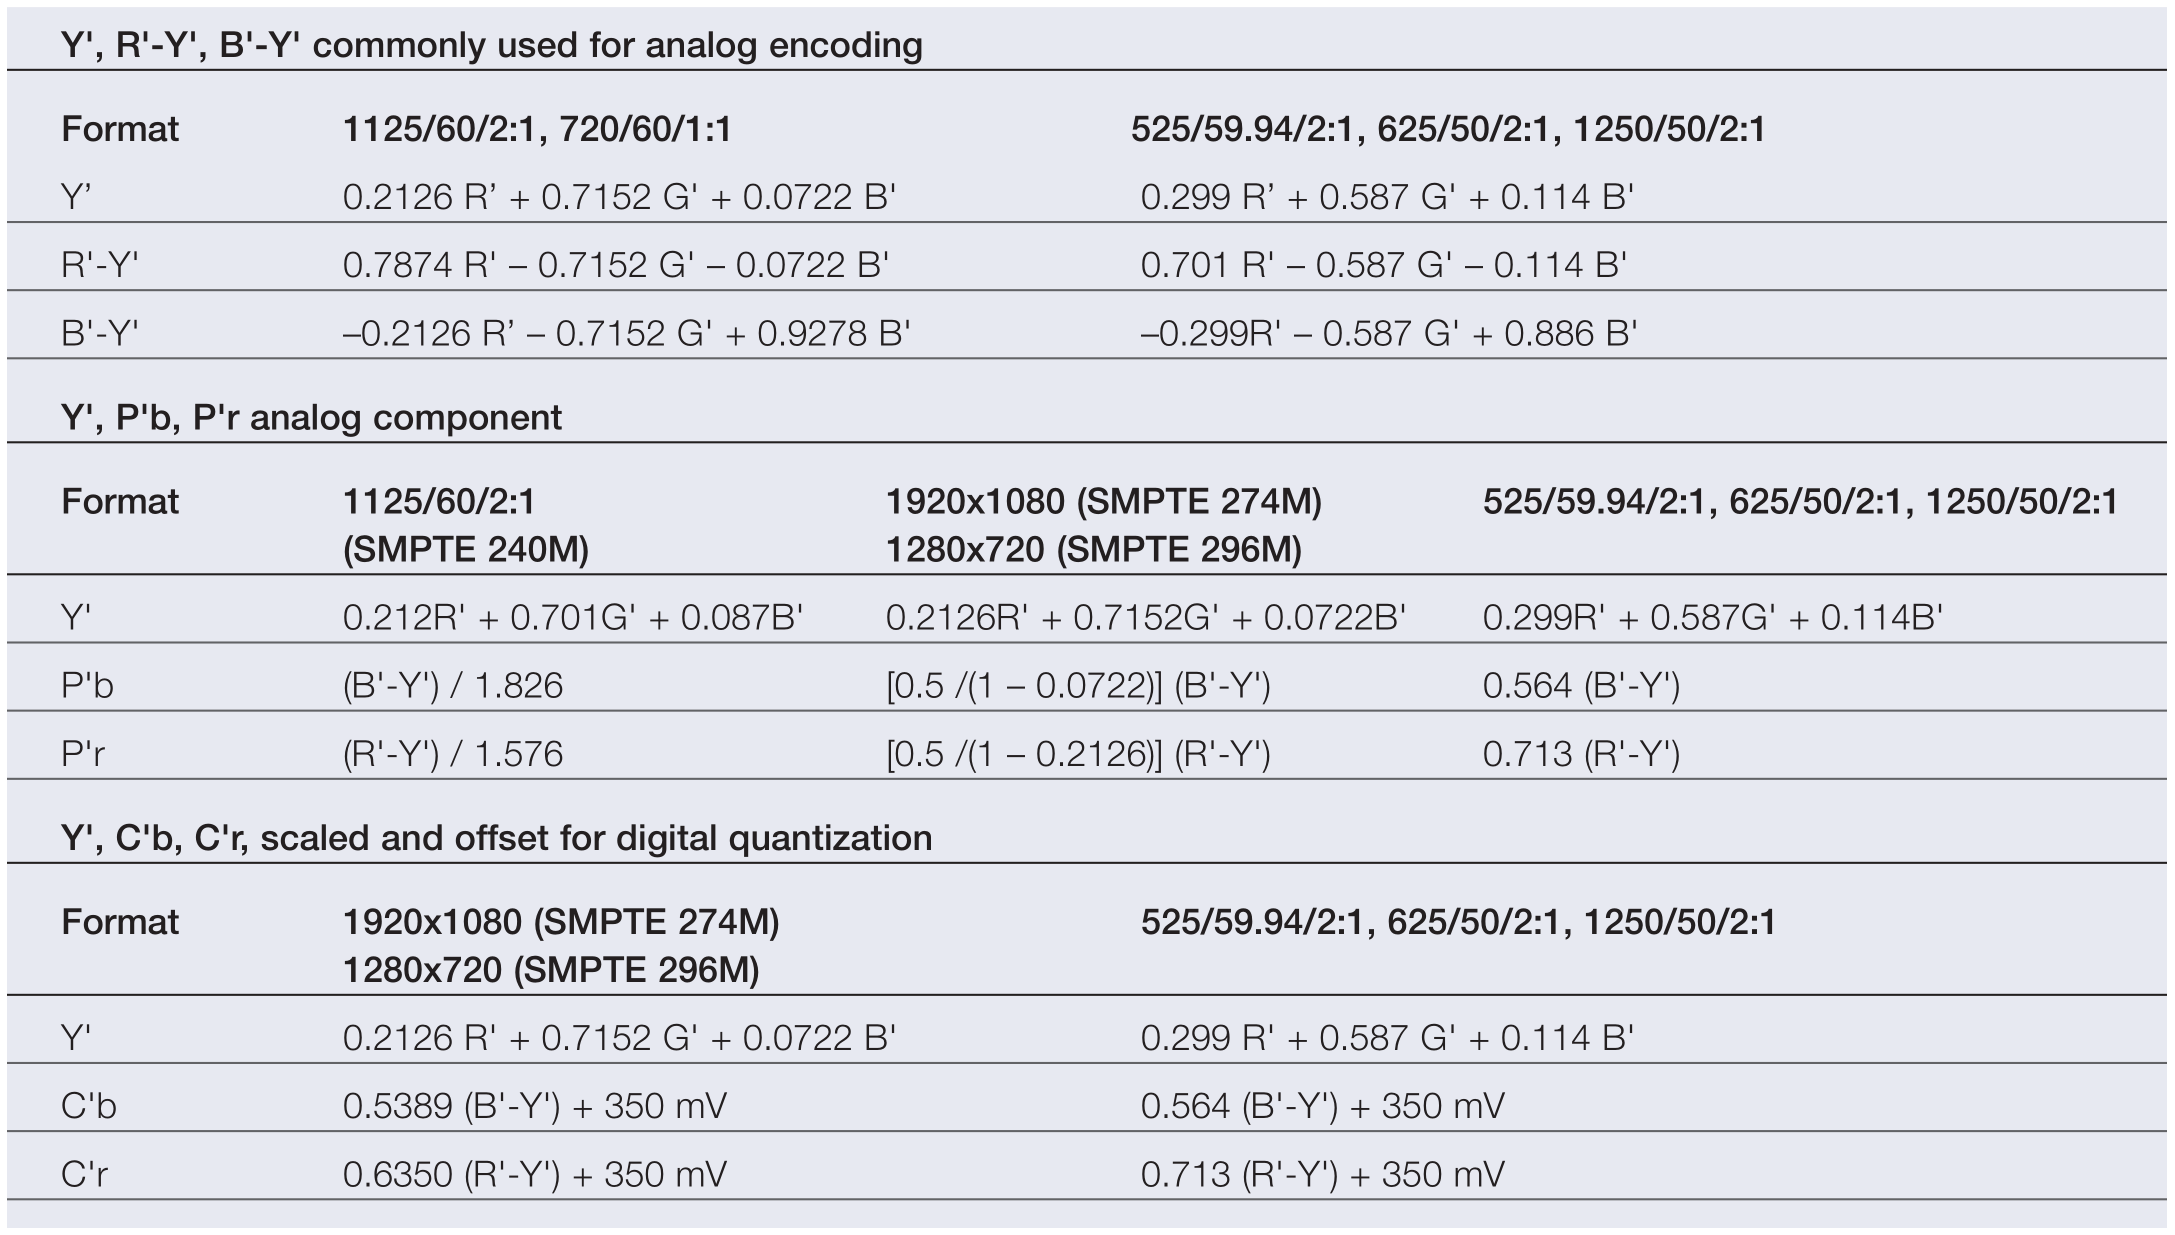
\includegraphics[width=\textwidth]{luma and chroma components.PNG}
    \caption{휘도와 색상 비디오 요소}\label{table:luma and chroma components}
\end{tab*}
감마 보정된 R'G'B' 요소들은 행렬을 이용해서 감마 보정된 휘도(Y')와 두 개의 색차 요소로 바뀐다. 휘도와 색차 요소들은 표 \ref{table:table 1}에 나온 값들을 이용해서 R',G',B'로부터 나온다(각 계수들의 단위는 볼트이다).
\\
표 \ref{table:luma and chroma components}\은 R'G'B'에서 Y',(R'-Y'),(B'-Y')로의 변환에 사용되는 전압의 범위를 알려준다. 휘도 신호는 0에서 700 mV의 다이내믹 레인지를 갖는다.
색차 신호들인 R'-Y'와 B'-Y'는 여러 요소 포맷들에 따라 달라지는 배율에 의해 다른 다이내믹 레인지를 가질 수 있다. Y'P'bP'r로 표기되는 아날로그 요소 포맷에서는 두 색차 값은 $\pm 350$ mV의 다이내믹 레인지를 갖는다. 이는 비디오 신호 처리를 더 단순하게 해준다.
아날로그 Y'Pb'Pr' 값은 오프셋이 더해져서 디지털 표준에서 보통 사용되는 Y'C'bC'r이 된다. 이로부터 나오는 비디오 요소들은 흑백 비디오 신호와 비슷한 Y' 또는 휘도 채널과 두 개의 색차 채널인 C'b와 C'r인데 이들은 밝기 정보 없이 색상 정보만 전달하며 이 세 신호는 모두 디지털 데이터로 변환되기 적절하게 배율이 곱해진다.
\\
\begin{tab}[hpb!]
    \centering
    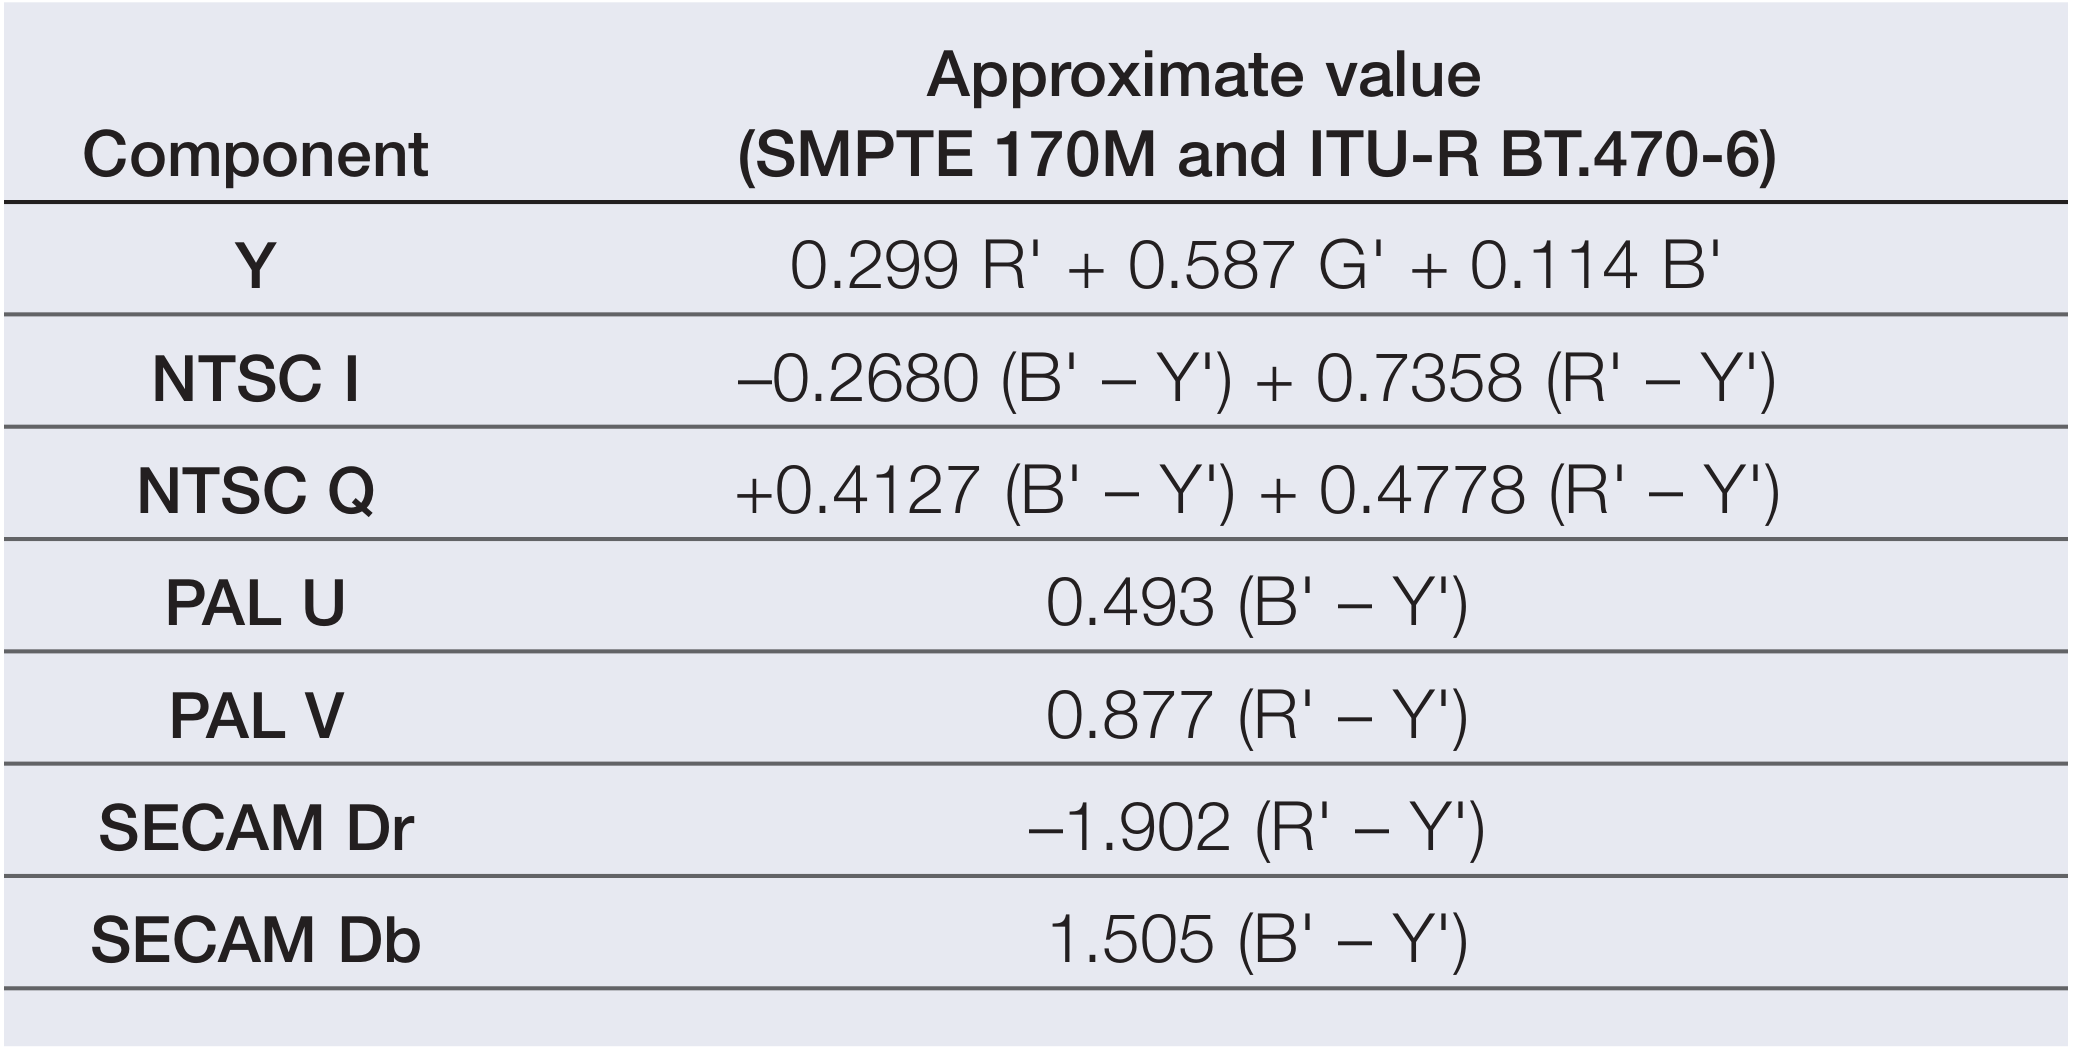
\includegraphics[width=0.5\textwidth]{luma and chroma for composite encoding.PNG}
    \caption{컴포지트 비디오 인코딩을 위한 휘도와 색차 값}\label{table:luma and chroma for composite encoding}
\end{tab}
여러 다른 색차 포맷들이 다양한 상황에서 사용된다. 컴포지트 PAL, SECAM과 NTSC 인코딩에서 현재 사용되는 계수 값들이 표 \ref{table:luma and chroma for composite encoding}에 나와 있는 것처럼 다르다는 것을 아는 것은 특히 중요하다.
